\documentclass[11pt]{article}

\usepackage{hyperref}
\usepackage{mathtools}
\usepackage{amsthm}
\usepackage{amssymb}
\usepackage{MnSymbol}
\usepackage{mathrsfs}
\usepackage[arrow]{xy}
\usepackage{tikz}
\usepackage{dsfont}
\usepackage{enumitem}
\usepackage{accents}
\usepackage{tabu}
\usepackage{setspace}

\pagestyle{headings}

\newcommand{\Z}{\mathbb{Z}}

\newtheoremstyle{mythm} % name of style
	{\topsep} % spacing above thm env
	{\topsep} % spacing below thm env
	{\singlespacing} % name of font and spacing to use in body of them env
	{0pt} % indent spacing
	{\bfseries} % name of head font
	{.} % punctuation between head and body
	{5pt plus 1pt minus 1pt} % space after thm head; " " = normal interword space
	{} % head specification
	
\theoremstyle{mythm}
\newtheorem{defn}{Definition}[section]
\newtheorem{ex}[defn]{Example}
\newtheorem{theo}[defn]{Theorem}
\newtheorem{prop}[defn]{Proposition}
\newtheorem{lem}[defn]{Lemma}
\newtheorem{que}[defn]{Question}
\newtheorem*{conj}{Conjecture}

\begin{document}

\author{Stephen Shang Yi Liu}
\title{On the asymptotic behavior of the magnitude function for odd-dimensional Euclidean balls}
\date{}

\maketitle

\begin{abstract}
Magnitude is a numerical invariant of metric spaces with origins in the notion of the Euler characteristic of a category. To this day the only convex sets in Euclidean space for which we can compute magnitude are the odd-dimensional Euclidean balls. Recent results have shed light on the asymptotic behavior of the magnitude function for these Euclidean balls, and in particular recent work by Meckes showed that the first order small-$t$ asymptotics of the magnitude function recovers its first intrinsic volume. The aim of this thesis is to survey work done to understand the magnitude function for odd-dimensional Euclidean balls and to compute its second order small-$t$ asymptotics.
\end{abstract}

\newpage

\tableofcontents

\newpage

\section{Introduction}

Magnitude is a numerical invariant of metric spaces. Its precursor is the Euler characteristic of a finite category, introduced by Leinster in \cite{leinster_euler_2006} as an analog to the classical notion of the Euler characteristic of a topological space. In \cite{leinster_magnitude_2011}, Leinster extended his definition of the Euler characteristic of a finite category to finite enriched categories. An enriched category $\mathscr{C}$ is one where the hom-sets of any two objects in $\mathscr{C}$ are in fact objects of some monoidal category $\mathscr{V}$. Lawvere observed that categories enriched in $([0,\infty],0,\leq)$ can be seen as generalized metric spaces where for any two objects $a,b$, the hom-set $\text{Hom}(a,b) \in [0,\infty]$ gives the distance between $a,b$ satisfying the triangle identity. This notion of distance is more general than in a classical metric space because distances are allowed to be infinite and may no longer be symmetric. Taking the definition of the Euler characteristic of a finite category enriched in $[0,\infty]$ we arrive at the definition of magnitude for a finite metric space.

Soon after defining magnitude for finite metric spaces, Leinster and others considered the question of defining magnitude for infinite metric spaces. Willerton in \cite{willerton_heuristic_2009} computed the magnitudes of some infinite sets via approximation by finite subsets, though at this point it was not clear whether such computations were independent of the approximations chosen. Meckes in \cite{meckes_positive_2013} showed that defining magnitude for infinite metric spaces via approximations by finite subsets is indeed consistent for a special class of metric spaces: the compact positive definite metric spaces. In addition, Meckes showed that one can arrive at an equivalent definition that extends to compact metric spaces (see \cite{meckes_magnitude_2015} and \cite{leinster_magnitude_2017}.

However, at this point, there are only a few spaces for which magnitude is known exactly. Among them include:
\begin{enumerate}[label=\arabic*.]
\item Compact intervals in $\mathbb{R}$ (\cite{leinster_magnitude_2017}),
\item $n$-spheres with the intrinsic metric (\cite{willerton_magnitude_2014}),
\item Compact $\ell_1$-convex sets in $\ell_1^n$ (\cite{leinster_magnitude_2017}),
\item odd-dimensional Euclidean balls (\cite{barcelo_magnitudes_2016} and \cite{willerton_magnitude_2017}).
\end{enumerate}

Leinster and Willerton in \cite{leinster_asymptotic_2013} conjectured that magnitude is a valuation on convex bodies. By computing the magnitude functions of odd-dimensional Euclidean balls in dimensions 3, 5, and 7, Barcelo and Carbery showed in \cite{barcelo_magnitudes_2016} that this convex magnitude conjecture is false, however, recent work by Willerton, Gimperlein and Goffeng, and Meckes in \cite{willerton_magnitude_2017}, \cite{gimperlein_magnitude_2017}, and \cite{meckes_magnitude_2019} respectively showed evidence for various asymptotic versions of the convex magnitude conjecture.

The goal of this thesis is to survey these results and to extend work by Meckes in \cite{meckes_magnitude_2019} to investigate the second order small-$t$ asymptotics of the magnitude function for odd-dimensional Euclidean balls. Chapters 2 and 3 introduces the theory of magnitude for finite and infinite metric spaces respectively. Chapter 4 surveys results regarding the magnitude of odd-dimensional Euclidean balls. Chapter 5 and 6 are devoted to computing the second order small-$t$ asymptotics of the magnitude function for odd-dimensional Euclidean balls, reducing the computation to a counting problem that has been partially solved.

\section{Finite metric spaces}

We begin by introducing the theory of magnitude for finite metric spaces. See \cite{leinster_magnitude_2011} for a more comprehensive introduction.

\subsection{The magnitude of a finite metric space}

We start with the notion of the magnitude of a matrix. Let $M \in M_n(\mathbb{R})$. The vector $w \in \mathbb{R}^n$ is called a \textbf{weighting} if $Mw = 1_n$, the vector of all $1$'s. Similarly, $v \in \mathbb{R}^n$ is called a \textbf{coweighting} if $v^\star M = 1_n^\star$. The following lemma ensures that if a matrix $M$ admits both a weighting and a coweighting, then the sum of all the entries of the (co)weighting is independent of the (co)weighting chosen:

\begin{lem}\label{lem:indepweighting}
If $M$ has a weighting $w$ and a coweighting $v$, then $\sum\limits_{j=1}^{n}w_j = \sum\limits_{j=1}^{n}v_j$.
\end{lem}

\begin{proof}
\begin{equation*}
\sum\limits_{j=1}^{n}w_j = 1_n^\star w = v^\star Mw = v^\star 1_n = \sum\limits_{j=1}^{n}v_j.
\end{equation*}
\end{proof}

The lemma allows us to define the magnitude of a matrix. Let $M \in M_n(\mathbb{R})$. If $M$ has a weighting $w$ and a coweighting $v$, then we say $M$ has \textbf{magnitude} and its magnitude is given by
\begin{equation*}
\vert M \vert = \sum\limits_{j=1}^{n} w_j = \sum\limits_{j=1}^{n}v_j.
\end{equation*}

It is not obvious how to find the weighting of a matrix (if it exists at all), but the situation is more straightforward if the matrix is invertible:

\begin{lem}\label{lem:inv}
If $M \in M_n$ is invertible, then it has a unique weighting and coweighting and $\vert M \vert = \sum\limits_{i,j=1}^{n}[M^{-1}]_{ij}$
\end{lem}

\begin{proof}
If $M$ is invertible, then the equations
\begin{equation*}
Mx = 1_n, \quad x^\star M = 1_n^\star
\end{equation*}
have unique solutions which give the weighting and coweighting of $M$ respectively. In particular, the weighting $w$ is given by
\begin{equation*}
w = M^{-1}1_n = \sum\limits_{j=1}^{n} a_j^{-1}
\end{equation*}
where $a_j^{-1}$ is the $j$-th column of $M^{-1}$. Then the magnitude of $M$ is given by
\begin{equation*}
\sum\limits_{j=1}^{n}w_j = \sum\limits_{i=1}^{n}\sum\limits_{j=1}^{n}a_{j}^{-1}(i) = \sum\limits_{i,j=1}^{n}[M^{-1}]_{ij}
\end{equation*}
where $a_{j}^{-1}(i)$ denotes the $i$-th entry of $a_j^{-1}$.
\end{proof}

Now that we have the matrix preliminaries established we can move on to the definition of the magnitude of a finite metric space. Let $A$ be a finite metric space with $n$ points and distance function $d$. Then the \textbf{similarity matrix} $Z_A$ is the $n\times n$ real matrix given by $[Z_A]_{ij} = e^{-d(i,j)}$ where $i,j \in A$. The \textbf{magnitude} of $A$ is the magnitude of its similarity matrix, assuming it has a defined magnitude. We also denote the magnitude of $A$ by $\vert A\vert$.

We now present some basic examples of metric spaces and their magnitudes:

\begin{ex}
\begin{enumerate}
\item Let $A$ be the discrete metric space, that is, $d(a,b) = \infty$ for all $a \neq b$ in $A$. Then the similarity matrix $Z_A$ is the identity matrix and so $\vert A \vert = \#A$ where $\#A$ is the number of points in $A$.
\item Let $A$ be the metric space of two points $a,b$ and let $d = d(a,b)$. Then we have the similarity matrix
\begin{equation*}
Z_A = \begin{bmatrix} 1 & e^{-d} \\ e^{-d} & 1 \end{bmatrix}
\end{equation*}
which is invertible with inverse matrix given by
\begin{equation*}
Z_A^{-1} = \begin{bmatrix} \frac{1}{1-e^{-2d}} & \frac{-e^{-d}}{1-e^{-2d}} \\ \frac{-e^{-d}}{1-e^{-2d}} & \frac{1}{1-e^{-2d}} \end{bmatrix}
\end{equation*}
and so $A$ has magnitude
\begin{equation*}
\vert A \vert = \frac{2(1-e^{-d})}{1-e^{-2d}} = \frac{2(1-e^{-d})}{(1+e^{-d})(1-e^{-d})} = \frac{2}{1+e^{-d}} = 1+\tanh{\left(\frac{d}{2}\right)}.
\end{equation*}
\end{enumerate}
\end{ex}

\subsection{The magnitude function}

Given a finite metric space $A$, we have a one parameter family of matrices $tA$ where the distances in $A$ are scaled by a real parameter $t > 0$. Then we call the assignment $t\mapsto\vert tA \vert$ the \textbf{magnitude function} of $A$. Note that the metric space $tA$ does not necessarily admit a weighting for all values of $t$, so the magnitude function is a partially defined function from $(0,\infty)\to\mathbb{R}$.

Note that as we scale up distances between points, the metric space $A$ ``approaches" the discrete space and so we want to be able to say that $\vert tA \vert \to \#A$ as $t \to \infty$. Actually proving this statement is a little more tricky than it first seems because, as noted above, $\vert tA \vert$ is not necessarily defined for all $t$. To do this, we prove the following lemma and proposition. The lemma and proposition, along with their proofs, can be found in \cite{leinster_magnitude_2011} as Lemma 2.2.5 and Proposition 2.2.6.

A metric space $A$ is an \textbf{expansion} of a metric space $B$ if there exists a distance-decreasing surjection from $A$ to $B$, that is, there exists an $f: A \to B$ surjective such that for all $a,b \in A$, $d_{B}(f(a),f(b)) \leq d_{A}(a,b)$.

\begin{lem}\label{lem:expansion}
Suppose $A,B$ are both finite metric spaces with nonnegative weightings (that is, the entries of their respective weightings are nonnegative). Then if $A$ is an expansion of $B$, then $\vert A \vert \geq \vert B \vert$.
\end{lem}

\begin{proof}
Since $A$ is an expansion of $B$, there exists a distance decreasing surjection $f: A \to B$. Take a right-inverse function of $f$, say $g: B \to A$ (which we know exists since $f$ is surjective). Then for all $b \in B$, $f(g(b)) = b$ and so for all $a \in A$ and $b \in B$, we have
\begin{equation*}
d_{B}(f(a),b) = d_{B}(f(a),f(g(b))) \leq d_{A}(a,g(b))
\end{equation*}
this also means
\begin{equation*}
\left[Z_B\right]_{f(a),b} \geq \left[Z_{A}\right]_{a,g(b)}
\end{equation*}
(note the reversal of the direction in the inequality). Now let $w_A,w_B$ be respective nonnegative weightings. In what follows, we'll use functional notation $w_A(i)$ to denote the $i$-th entry of $w_A$ an similarly for $w_B$. Then by nonnegativity of the weighting and the inequality above, we have
\begin{align*}
\vert A \vert = \sum\limits_{a\in A} w_A(a) \cdot 1 &= \sum\limits_{a\in A, b\in B} w_A(a) \left[Z_{B}\right]_{f(a),b}w_B(b) \\
&\geq \sum\limits_{a\in A, b \in B} w_{A}(a) \left[Z_{A}\right]_{a,g(b)} w_{B}(b) = \sum\limits_{b\in B} 1\cdot w_B(b) = \vert B \vert
\end{align*}
as required.
\end{proof}

\begin{prop}\label{prop:approach}
Let $A$ be a finite metric space. Then
\begin{enumerate}[label=(\roman*)]
\item $tA$ is invertible and hence has magnitude for all but finitely many $t > 0$.
\item The magnitude function of $A$ is analytic at all $t>0$ such that $tA$ is invertible.
\item for $t \gg 0$, there is a unique, positive, weighting on $tA$.
\item For $t \gg 0$, the magnitude function of $A$ is increasing.
\item $\vert tA \vert \to \#A$ as $t \to \infty$.
\end{enumerate}
\end{prop}

\begin{proof}
Let $\#A = n$. For an $n \times n$ invertible matrix $M$, by Lemma \ref{lem:inv}, the unique weighting $w$ on $M$ is given by
\begin{equation}
w_i = \sum\limits_{j=1}^{n}\left[M^{-1}\right]_{ij}.
\end{equation}
We can rewrite (1) in terms of the adjugate and the determinant of $M$:
\begin{equation}
w_i = \sum\limits_{j=1}^{n}\left[M^{-1}\right]_{ij} = \sum\limits_{j=1}^{n} \frac{\left[\text{adj}(M)\right]_{ij}}{{\det{M}}}
\end{equation}
where $M\text{adj}(M) = (\det{M})I_n$. Note that the adjugate is a smooth function of $M$ (see section 0.8 of \cite{horn_matrix_2013}).

To show $\emph{(i)}$, note that since $Z_{tA} \to I_n$ as $t\to\infty$ and $I_n$ is invertible, $Z_{tA}$ is invertible for large enough $t$. Also note that $\det{Z_{tA}}$ is analytic in $t$. One way to see this is by looking at the Liebniz formula for the determinant found in \cite{horn_matrix_2013} applied to our definition of the similarity matrix:
\begin{equation*}
\det{Z_{tA}} = \sum\limits_{\sigma} \text{sgn}(\sigma)\prod\limits_{a\in A}\left[Z_{tA}\right]_{a,\sigma(a)} = \sum\limits_{\sigma}\text{sgn}(\sigma)\prod\limits_{a\in A} e^{-td(a,\sigma(a))}
\end{equation*}
where $\sigma$ is a permutation of $n$ elements. From the formula above, clearly the determinant is analytic in $t$ (it is the sum and product of analytic functions). Then since $Z_{tA} \to I_n$ as $t \to\infty$ and $\det I_n$ = 1, $\det Z_{tA} > 0$ for large enough $t$, and so by analyticity, $\det Z_{tA}$ has finitely many zeroes for $t \in (0,\infty)$.

For $\emph{(ii)}$, since magnitude is the sum of all the entries in the weighting, analyticity of the magnitude function for all $t > 0$ such that $tA$ is invertible follows from Equation (2) and analyticity of the quotient.

For $\emph{(iii)}$, fix $a \in A$ and note that by Equation (2), the function $Z_{tA} \mapsto w_{tA}(a)$ is continuous on the space of $n \times n$ invertible matrices (where $w_{tA}$ denotes the weighting on $Z_{tA}$). Now, $w_{I_n}(a) = 1$, so by continuity since $Z_{tA}$ converges to $I_n$ as $t \to \infty$, the weighting $w_{tA}(a)$ is also positive for large enough $t$. In other words, $Z_{tA}$ has a positive weighting for large enough $t$.

To show $\emph{(iv)}$, let $t \leq t'$. Note that by part $\emph{(iii)}$, $tA$ and $t'A$ have positive weightings for large enough $t$. Note also that $t'A$ is an expansion of $tA$ (taking the function $f:tA \to t'A$ to be the identity as a map of sets as our distance decreasing surjection). So applying Lemma \ref{lem:expansion} above, we see that the magnitude function is increasing for $t \gg 0$.

Finally for $\emph{(v)}$, by everything above, we have that $\lim\limits_{t\to\infty} \vert tA \vert = \left\vert \lim\limits_{t\to\infty}Z_{tA}\right\vert = \vert I_n\vert = n = \#A$.
\end{proof}

So for any finite metric space $A$, the value of the magnitude function approaches the cardinality of $A$ as we blow up distances between points. However, along with the fact that the magnitude may not be defined everywhere, other ``nice'' properties that we might expect, such as monotonicity or non-negativitiy, are not guaranteed for the magnitude function, as the following example shows:

\begin{ex}
Let $K_{3,2}$ be the graph with vertices $a_1,a_2,a_3$ and $b_1,b_2$ and one edge between $a_i$ and $b_j$ for each $i$ and $j$. Let each edge have length $t$. The distance function on $K_{3,2}$ is the shortest path distance in the graph (see Figure \ref{fig:K32}).

\begin{figure}[h!]
\begin{equation*}
\begin{xy}
(0,0)*+{\bullet_{a_1}}="a1";
(0,-20)*+{\bullet_{a_2}}="a2";
(0,-40)*+{\bullet_{a_3}}="a3";
(60,-10)*+{\bullet_{b_1}}="b1";
(60,-30)*+{\bullet_{b_2}}="b2";
{\ar@{-} "a1";"b1"}?*!/_3mm/{t};
{\ar@{-} "a2";"b1"};
{\ar@{-} "a3";"b1"};
{\ar@{-} "a1";"b2"};
{\ar@{-} "a2";"b2"};
{\ar@{-} "a3";"b2"};
\end{xy}
\end{equation*}
\caption{\label{fig:K32}The graph $K_{3,2}$.}
\end{figure}

Then for each $t$, we can compute the similarity matrix and the magnitude:

\begin{equation*}
Z_{tK_{3,2}} = \begin{bmatrix} 1 & e^{-2t} & e^{-2t} & e^{-t} & e^{-t} \\
e^{-2t} & 1 & e^{-2t} & e^{-t} & e^{-t} \\
e^{-2t} & e^{-2t} & 1 & e^{-t} & e^{-t} \\
e^{-t} & e^{-t} & e^{-t} & 1 & e^{-2t} \\
e^{-t} & e^{-t} & e^{-t} & e^{-2t} & 1
\end{bmatrix} \qquad
\vert tK_{3,2} \vert = \frac{5-7e^{-t}}{(1+e^{-t})(1-2e^{-2t})}
\end{equation*}

\begin{figure}[h!]
\centerline{
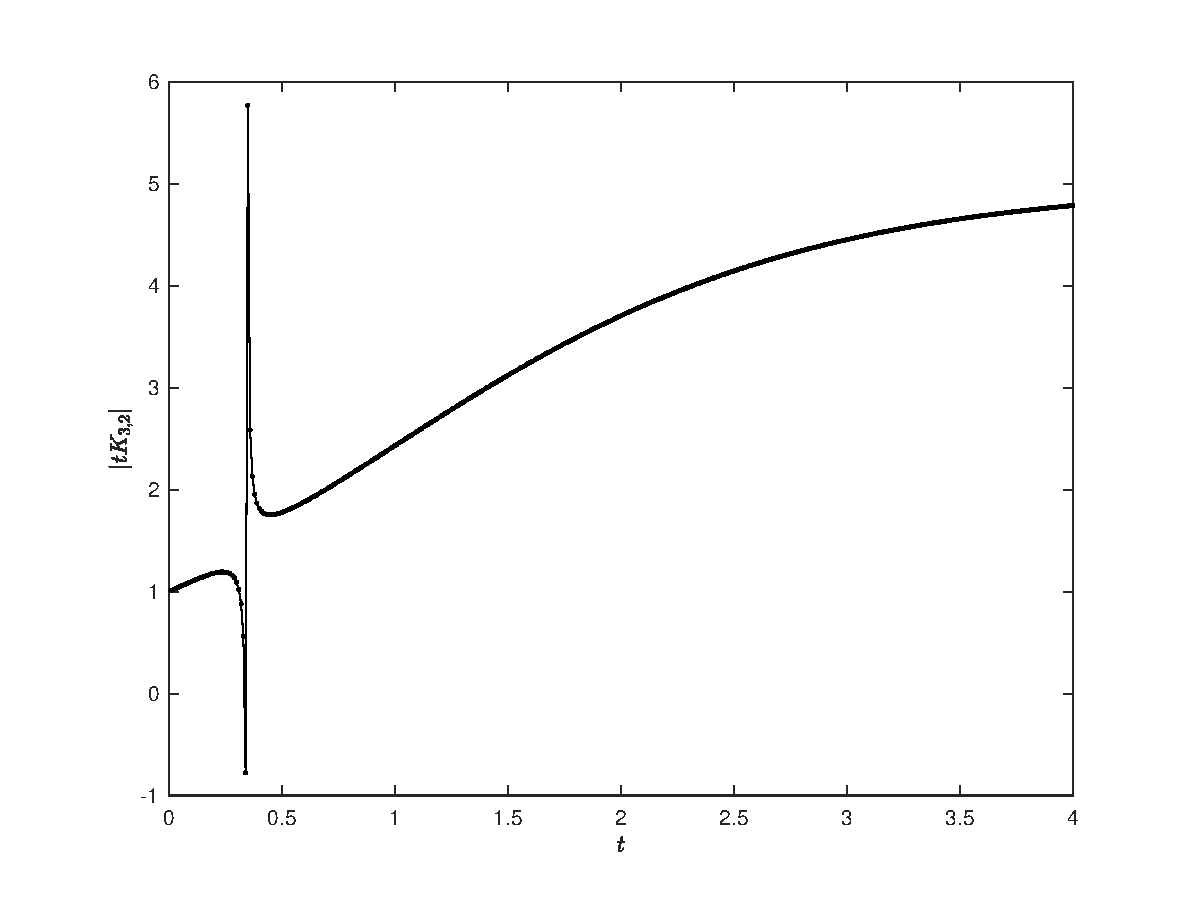
\includegraphics[width=10cm]{K32.eps}}\caption{\label{fig:K32magfun}The magnitude function of $K_{3,2}$.}
\end{figure}

The graph of the magnitude function for $K_{3,2}$ shows how pathological the magnitude function of a metric space can be (see Figure \ref{fig:K32magfun}). In particular,
\begin{enumerate}[label=\arabic*.]
\item it is undefined for $t = \log{\sqrt{2}}$,
\item there are values for which it is negative,
\item it is not monotonic,
\item and finally it can exceed the cardinality of $K_{3,2}$.
\end{enumerate}
\end{ex}

\subsection{Finite positive definite metric spaces}

Given the example above, it is natural to ask whether there are classes of finite metric spaces for which the magnitude function is more well-behaved. The metric spaces with positive definite similarity matrix are one such class. We say a finite metric space $A$ is \textbf{positive definite} if its similarity matrix $Z_A$ is a positive definite matrix. Since positive definite matrices are invertible, any positive definite metric space has magnitude. Likewise, since prinicipal submatrices of positive definite matrices are positive definite, subspaces of positive definite metric spaces are positive definite and hence also have magnitude.

The main attractiveness of positive definite metric spaces is that magnitude is guaranteed to be defined, and we have a more convenient explicit formula for the magnitude:

\begin{prop}\label{prop:finiteposdefsup}
If $A$ is a positive definite metric space, then $A$ has magnitude and
\begin{equation*}
\vert A \vert = \sup\limits_{v \neq 0}\frac{\left(\sum_{a\in A}v_a\right)^2}{v^\star Z_Av}
\end{equation*}
where $v \in \mathbb{R}^{\#A}$. $v$ attains the supremum if and only if it is a nonzero scalar multiple of the unique weighting on $A$.
\end{prop}

\begin{proof}
Since $Z_A$, we have the Cauchy-Schwarz inequality:
\begin{equation*}
(v^\star Z_A w)^2 \leq (v^\star Z_Av)(w^\star Z_Aw)
\end{equation*}
with equality if and only if $v,w$ are scalar multiples of each other. We take $w$ to be the unique weighting on $Z_A$. Then we have
\begin{equation*}
\vert A \vert = \sum\limits_{a\in A}w_a = w^\star Z_Aw \geq \frac{(v^\star Z_Aw)^2}{v^\star Z_Av} = \frac{\left(\sum_{a\in A}v_a\right)^2}{v^\star Z_Av}
\end{equation*}
for all $v$. So $\vert A \vert$ is greater than or equal to the supremum. But taking $w$ to be the unique weighting gives
\begin{equation*}
\frac{\left(\sum_{a\in A}w_a\right)^2}{w^\star Z_Aw} = \frac{(w^\star Z_Aw)^2}{w^\star Z_Aw} = w^\star Z_Aw = \sum\limits_{a\in A}w_a = \vert A \vert
\end{equation*}
so we have equality.
\end{proof}

Using this formulation of the magnitude, we can show some that magnitude is increasing with respect to inclusion for positive definite metric spaces.

\begin{prop}\label{prop:finiteposdefincreasing}
If $A$ is a positive definite metric space and $B \subseteq A$, then $\vert B \vert \leq \vert A \vert$.
\end{prop}

\begin{proof}
As mentioned above, since $A$ is positive definite and $B$ is a subspace of $A$, $B$ is also positive definite and so has magnitude. Then we have
\begin{equation*}
\vert B \vert = \sup\limits_{v\neq0}\frac{(\sum_{b\in B} v_b)^2}{v^\star Z_Bv} \leq \sup\limits_{v\neq0}\frac{(\sum_{a\in A}v_a)^2}{v^\star Z_Av} = \vert A\vert
\end{equation*}
since the space of vectors we are considering for $B$ is a subset of the space of vectors we consider for $A$ (after embedding $\mathbb{R}^{\#B}$ into $\mathbb{R}^{\#A}$).
\end{proof}

\section{Infinite metric spaces}

Now we move on to the theory of magnitude for more general classes of metric spaces. Two strategies that naturally arise for generalizing magnitude for finite spaces to infinite spaces would be to either approximate infinite metric spaces by finite subspaces, or to generalize the notion of a weighting to an infinite setting. Meckes in \cite{meckes_positive_2013} defined magnitude for the class of compact positive definite metric spaces that is reminiscent of the formula given in Proposition \ref{prop:finiteposdefsup}, and showed that it agrees with the definition that arises out of approximating by finite subspaces. However, this only defined magnitude for positive definite spaces, and Meckes in \cite{meckes_magnitude_2015} gave a definition of magnitude for more general compact metric spaces. We briefly survey these results (without proofs) in the section below. A more comprehensive survey can be found in \cite{leinster_magnitude_2017}.

\subsection{Compact positive definite metric spaces}

Let $A$ be a metric space. We say $A$ is a \textbf{positive definite metric space} if every finite subspace of $A$ is positive definite. The property that $tA$ is a positive definite metric space for all $t > 0$, is equivalent to the property that $A$ is of \textbf{negative type}. Several well-known metric spaces are of negative type, and we will later see that they have well-defined magnitudes.

We begin with the strategy of approximating by finite subspaces. To approximate, we need to have a topology on the class of compact metric spaces. Let $X$ be a metric space. Then the \textbf{Hausdorff metric} $d_H$ on the class of compact subsets $A,B$ is given by
\begin{equation*}
d_H(A,B) = \max\{\sup\limits_{a\in A}d(a,B),\sup\limits_{b\in B}d(b,A)\}
\end{equation*}
where $d$ is the distance function on $X$. By considering embeddings of compact metric spaces into ambient spaces, we have a notion of distances between two metric spaces: the \textbf{Gromov-Hausdorff distance} between two compact metric spaces $A,B$ is given by
\begin{equation*}
d_{GH}(A,B) = \inf d_H(\varphi(A),\psi(B))
\end{equation*}
where the infimum is over all metric spaces $X$ and isometric embeddings $\varphi:A \to X$ and $\psi: B \to X$.

The following proposition allows us to define the magnitude of a compact positive definite metric space via approximations by finite positive definite spaces:

\begin{prop}[Proposition 3.1 of \cite{leinster_magnitude_2017}]\label{prop:MAlsc}
The quantity
\begin{equation*}
M(A) = \sup\{\vert A'\vert : A' \subseteq A, \text{$A'$ finite}\}
\end{equation*}
is a lower semicontinuous function of $A$ (taking values in $[0,\infty]$) in the class of compact positive definite metric spaces equipped with the Gromov-Hausdorff topology.
\end{prop}

Let $A$ be a compact positive definite metric space. We can therefore define the \textbf{magnitude of a compact positive definite metric space} $\vert A \vert$ to be the supremum of $M(A)$. Semicontinuity and Proposition \ref{prop:finiteposdefincreasing} ensures that if $A$ is finite, then $M(A) = \vert A \vert$, so this new definition agrees with magnitude for the finite case. Furthermore, the magnitude of $A$ is independent of the choice of approximating sequence of finite subsets:

\begin{prop}[Proposition 3.3 of \cite{leinster_magnitude_2017}]\label{prop:finiteapprox}
Let $A$ be a compact positive definie metric space, and let $\{A_k\}$ be any sequence of compact subsets of $A$ such that $A_k\to A$ in the Hausdorff topology. Then $\vert A \vert = \lim\limits_{k\to\infty}\vert A_k\vert$.
\end{prop}

Recall that $A$ is of negative type if $tA$ is positive definite for all $t > 0$. Then by above all compact subsets of $A$ have a well-defined (possibly infinite) magnitude. In particular, the following spaces are known to be of negative type and hence have magnitude (Theorem 2.11 of \cite{leinster_magnitude_2017} and Theorem 3.6 of \cite{meckes_positive_2013}):

\begin{enumerate}[label=\arabic*.]
\item $\ell^n_p$ for $n\geq1$ and $1\leq p \leq 2$,
\item $L_p[0,1]$ for $1\leq p \leq 2$,
\item $n$-spheres with the geodesic distance,
\item weighted trees.
\end{enumerate}

Willerton in \cite{willerton_magnitude_2014} gives an explicit formula for the magnitude of $n$-spheres with the intrinsic metric.

\subsection{Compact metric spaces}

To extend the definition of magnitude to compact metric spaces, we need to generalize the notion of a weighting. Let $A$ be a compact metric space and let $\mu$ be a finite signed Borel measure on $A$. We say $\mu$ is a \textbf{weight measure} on $A$ if
\begin{equation*}
\int_A e^{-d(a,b)}d\mu(b) = 1
\end{equation*}
for all $a \in A$.

Note that if $A$ is finite, then the vector $w \in \mathbb{R}^{\# A}$ given by
\begin{equation*}
w_a = \mu(\{a\})
\end{equation*}
is a weighting of $A$, and the magnitude is given by
\begin{equation*}
\vert A \vert = \sum\limits_{a\in A} w_a = \sum\limits_{a \in A} \mu(\{a\}) = \mu(A).
\end{equation*}

Hence we define the \textbf{magnitude of a compact metric space} $A$ to be $\vert A \vert = \mu(A)$. If $A$ is compact positive definite, then this definition agrees with the definition of magnitude given in the previous section (Proposition 3.6 of \cite{leinster_magnitude_2017}). Moreover, using this definition, we have an explicit formula for the magnitude that is reminiscent of Proposition \ref{prop:finiteposdefsup}:

\begin{prop}[Theorems 2.3 and 2.4 of \cite{meckes_positive_2013}]\label{prop:variationalformula}
Let $A$ be a compact positive definite metric space, then
\begin{equation*}
\vert A \vert = \sup\limits_{\mu \in FM(A)}\left\{\frac{\mu(A)^2}{\int_A \int_A e^{-d(a,b)}d\mu(a)d\mu(b)}: \int_A \int_A e^{-d(a,b)}d\mu(a)d\mu(b)\neq0\right\},
\end{equation*}
where $FM(A)$ denotes the space of finite signed Borel measures on $A$. The supremum is attained when we take scalar multiples of the weight measure of $A$, provided $A$ possesses one.
\end{prop}

\section{Odd-dimensional Euclidean balls}

We now briefly survey, without proofs, results regarding the magnitude and magnitude function of odd-dimensional Euclidean balls. These results hinge on the formulation of magnitude in terms of potential theory and capacities of sets Meckes introduced in \cite{meckes_magnitude_2015} in defining magnitude for general compact metric spaces. We begin with a statement of the erstwhile convex magnitude conjecture, as it motivates many of the results in this section.

Let $d = 2m+1$ where $m$ is a natural number. Denote by $B_2^d$ the $d$-dimensional closed Euclidean ball and $tB_2^d$ the $d$-dimensional ball with radius $t$ for $t > 0$.

\subsection{The convex magnitude conjecture}

Let $\mathcal{K}^n$ be the space of compact convex sets in $\mathbb{R}^n$. We call a nonempty set in $\mathcal{K}^n$ a \textbf{convex body}. A \textbf{valuation} is a function $P:\mathcal{K}^n \to\mathbb{R}$ that satisfies the inclusion-exclusion principle, that is:
\begin{enumerate}[label=$\bullet$]
\item $P(\emptyset) = 0$,
\item $P(A\cup B) = P(A) + P(B) - P(A\cap B)$
\end{enumerate}
whenever $A,B,A\cup B \in \mathcal{K}^n$ ($A\cap B$ is automatically in $\mathcal{K}^n$ whenever $A$ and $B$ are). Hadwiger's Theorem states that if a valuation $P$ is invariant under rigid motions and is continuous with respect to the Hausdorff metric, then there are canonical homogenous valuations $V_0,V_1,\dots,V_n$ such that $P$ can be written as a linear combination of these valuations. The valuations $V_i$ are called the $i$-th intrinsic volumes with $V_n$ being the usual $n$-dimensional volume, $V_{n-1}$ being half the surface area and $V_0$ is the Euler characteristic.

Computer calculations of the magnitudes of various sets in Euclidean space found in \cite{willerton_heuristic_2009} led to the following conjecture stated in \cite{leinster_asymptotic_2013}:

\begin{conj}[Leinster-Willerton]
Let $K\in\mathcal{K}^n$. Then magnitude is a valuation and moreover
\begin{equation*}
\vert K \vert = \sum\limits_{i\geq0}\frac{V_i(K)}{i!\omega_i}
\end{equation*}
where $V_i$ is the $i$-th intrinsic volume and $\omega_i$ is the volume of the unit ball in $\mathbb{R}^i$.
\end{conj}

By homogeneity of the intrinsic volumes, the conjecture is equivalent to
\begin{equation*}
\vert tK \vert = \sum\limits_{i\geq0}\frac{V_i(K)}{i!\omega_i}t^i.
\end{equation*}
That is, the magnitude function of a convex body is a polynomial in $t$ with coefficients proportional to the intrinsic volumes of $K$.

\subsection{Explicit magnitude functions for balls in low dimension}

Barcelo and Carbery in \cite{barcelo_magnitudes_2016} explicitly calculated the magnitude functions of Euclidean balls in dimensions 3,5,7:
\begin{align*}
&\text{Mag}(tB_2^3) = \frac{t^3}{3!}+t^2+2t+1 \\
&\text{Mag}(tB_2^5) = \frac{t^6+18t^5+135t^4+525t^3+1080t^2+1080t+360}{5!(t+3)} \\
&\text{Mag}(tB_2^7) = \frac{t^7}{7!} \\
&+ \frac{\frac{1}{180}t^9+\frac{2}{15}t^8+\frac{3}{2}t^7+\frac{31}{3}t^6+\frac{189}{4}t^5+145t^4+\frac{1165}{4}t^3+360t^2+240t+60}{t^3+12t^2+48t+60}
\end{align*}
So taking second derivatives and evaluating at $t = 0$, we have
\begin{align*}
&\frac{d^2}{dt^2}\text{Mag}(tB_2^3)\big\vert_{t=0} = 2 \\
&\frac{d^2}{dt^2}\text{Mag}(tB_2^5)\big\vert_{t=0} = \frac{38}{9} = 4.222\dots \\
&\frac{d^2}{dt^2}\text{Mag}(tB_2^7)\big\vert_{t=0} = \frac{162}{25} = 6.48 \\
\end{align*}

In particular, the magnitude function of $B_2^5$ provides an example of where the convex magnitude conjecture is false. However, there are partial results suggesting the convex magnitude conjecture holds asymptotically for small and large $t$.

\subsection{Schröder paths and large-$t$ asymptotics}

Willerton in \cite{willerton_magnitude_2017} gave an expression for the magnitude function of odd-dimensional balls in terms of collections of Schröder paths. We introduce them below:
\begin{defn}
\begin{enumerate}[label=$\bullet$]
\item A \textbf{Schröder path} is a finite directed path in the integer lattice in which each step $(x,y)\in\Z^2$ is either an \textbf{ascent} to $(x+1,y+1)$, a \textbf{descent} $(x-1,y-1)$ or a \textbf{flat step} $(x+2,y)$ (note the advance by \emph{two} spaces in the horizontal direction).
\item Fix $k\geq0$. A \textbf{disjoint k-collection} is a family of Schröder paths from $(-i,i)$ to $(i,i)$ for each $0\leq i\leq k$ such that no node in $\Z^2$ is contained in two of the paths (the paths are disjoint).
\item We denote by $X_k$ the set of all disjoint $k$-collections and by $X_k^j$ the set of disjoint $k$-collections with exactly $j$ flat steps.
\end{enumerate}
\end{defn}

When thinking about what kinds of disjoint $k$-collections we can have in $X_k^j$ for some fixed $j$, it is often useful to think about what a path needs to look like for increasing values of $i$. For example, consider the set $X_k^0$, that is, the set of disjoint $k$-collections with exactly 0 flat steps. At $i = 0$ we have the single dot at $(0,0)$ and at $i = 1$, since we are allowed no flat steps, the only possible path we can have is the path made up of one ascent followed immediately by one descent. Then for $i = 2$, the disjointness condition and the presence of the earlier path at height $i=1$ ensures that the only possible path we can have is the path made up of two ascents followed by two descents. We continue this argument for successive values of $i$. We will call the path at height $i$ consisting of $i$ ascents followed by $i$ descents a \textbf{V-path at height $i$} (because they look like upside down V's). So it turns out that $X_k^0$ consists only of one collection, denoted $\sigma_{\text{roof}}^k$, which is made up entirely of V-paths for each $0\leq i\leq k$.

Let $\sigma$ be a disjoint $k$-collection in $X_k$. For each path in $\sigma$ we associate a weighting to each step $\tau$ in the path by the following:
\begin{equation*}
\omega_j(\tau) = \begin{cases} 
1 &\text{if $\tau$ is an ascent,} \\
t &\text{if $\tau$ is a flat step,} \\
y+1-j &\text{if $\tau$ is a descent from height $y$ to height $y-1$.}
\end{cases}
\end{equation*}
For a collection $\sigma\in X_k$ the \textbf{(total) weight of $\sigma$}, denoted by $\omega_j(\sigma)$ is the product of all the weightings of each step of a path in $\sigma$, that is,
\begin{equation*}
\omega_j(\sigma) = \prod\limits_{\tau\in\sigma}\omega_j(\tau)
\end{equation*}
Note that if $\sigma \in X_k^\ell$, that is $\sigma$ has exactly $\ell$ flat steps, then $\omega_j(\sigma)$ will take the form $ct^\ell$ where $c$ is the product of all the weights on descents in $\sigma$. We will only use the weightings $\omega_0$ and $\omega_2$ for our purposes, that is, a descent starting at height $y$ will be weighted by either $y+1$ and $y-1$ respectively. Consider a V-path $\sigma$ at height $i$, then we have
\begin{align*}
&\omega_0(\sigma) = \frac{(2i+1)!}{(i+1)!} \\
&\omega_2(\sigma) = \frac{(2i-1)!}{(i-1)!}
\end{align*}
and since $\sigma_{\text{roof}}^k$ consists only of V-paths, we have
\begin{align*}
&\omega_0\left(\sigma_{\text{roof}}^k\right) = \prod\limits_{i=0}^k\frac{(2i+1)!}{(i+1)!} \\
&\omega_2\left(\sigma_{\text{roof}}^k\right) = \prod\limits_{i=1}^k\frac{(2i-1)!}{(i-1)!} \\
\end{align*}

\begin{figure}
\begin{equation*}
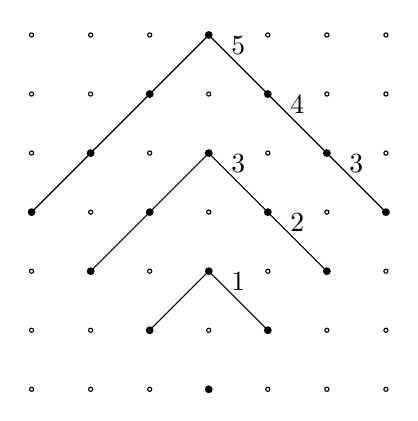
\begin{tikzpicture}[scale=0.75]
\foreach \i in {0,...,6}
	\foreach \j in {0,...,6}{
		\draw (\i,\j) circle(1pt);
	};
	
	% 0 level
	\node at (3,0) [circle, fill, inner sep=1pt]{};
	
	% 1 level
	\node at (2,1) [circle, fill, inner sep=1pt]{};
	\node at (4,1) [circle, fill, inner sep=1pt]{};
	\node at (3,2) [circle, fill, inner sep=1pt]{};
	\draw (2,1) -- (3,2);
	\draw (4,1) -- node[above] {1} (3,2);
	
	% 2 level
	\node at (1,2) [circle, fill, inner sep=1pt]{};
	\node at (2,3) [circle, fill, inner sep=1pt]{};
	\node at (3,4) [circle, fill, inner sep=1pt]{};
	\node at (4,3) [circle, fill, inner sep=1pt]{};
	\node at (5,2) [circle, fill, inner sep=1pt]{};
	\draw (1,2) -- (2,3) -- (3,4);
	\draw (3,4) -- node[above] {3} (4,3);
	\draw (4,3) -- node[above] {2} (5,2);
	
	% 3 level
	\node at (0,3) [circle, fill, inner sep=1pt]{};
	\node at (1,4) [circle, fill, inner sep=1pt]{};
	\node at (2,5) [circle, fill, inner sep=1pt]{};
	\node at (3,6) [circle, fill, inner sep=1pt]{};
	\node at (4,5) [circle, fill, inner sep=1pt]{};
	\node at (5,4) [circle, fill, inner sep=1pt]{};
	\node at (6,3) [circle, fill, inner sep=1pt]{};
	\draw (0,3) -- (1,4) -- (2,5) -- (3,6);
	\draw (3,6) -- node[above] {5} (4,5);
	\draw (4,5) -- node[above] {4} (5,4);
	\draw (5,4) -- node[above] {3} (6,3);
\end{tikzpicture}
\end{equation*}
\caption{\label{fig:Vpath} The disjoint 3-collection $\sigma^3_\text{roof}$ with $\omega_2$ weightings.}
\end{figure}

We are interested in these weightings on collections of Schröder paths because Willerton in \cite{willerton_magnitude_2017} showed the following:

\begin{theo}[Corollary 27 of \cite{willerton_magnitude_2017}]\label{theo:willertonND}
Let $d = 2m+1$ be odd. Then
\begin{equation*}
\text{Mag}\left(tB_2^d\right) = \frac{\sum\limits_{\sigma\in X_{m+1}}\omega_2(\sigma)}{d!\sum\limits_{\sigma\in X_{m-1}}\omega_0(\sigma)} = \frac{\sum\limits_{\sigma\in X_{m+1}}\prod\limits_{\tau\in\sigma}\omega_2(\tau)}{d!\sum\limits_{\sigma\in X_{m-1}}\prod\limits_{\tau\in\sigma}\omega_0(\tau)}
\end{equation*}
for all $t > 0$.
\end{theo}
As mentioned before, $\omega_j(\sigma)$ are of the form $ct^\ell$ where $\ell$ is the number of flat steps in $\sigma$ and $c$ is a constant, so the numerator and the denominator in the expression above are both polynomials in $t$. We will denote the function in the numerator by $N(t)$ and the function in the denominator (without the extra $d!$) by $D(t)$. Put more succinctly, we have
\begin{equation*}
\text{Mag}\left(tB_2^d\right) = \frac{N(t)}{d!D(t)}.
\end{equation*}

Using this combinatorial formulation of the magnitude function for the Euclidean ball, Willerton was able to determine the asymptotic behavior of the magnitude function as $t\to\infty$:

\begin{theo}[Corollary 30 of \cite{willerton_magnitude_2017}]\label{theo:largetasymptotics}
Let $d$ be odd. Then asymptotically, magnitude function of the $d$-dimensional Euclidean ball is given by
\begin{equation*}
\text{Mag}\left(tB_2^d\right) = \frac{1}{d!}\left(t^d + \frac{d(d+1)}{2}t^{d-1} + \frac{(d-1)d(d+1)^2}{8}t^{d-2}\right) + O(t^{d-2})
\end{equation*}
as $t\to\infty$.
\end{theo}

Gimperlein and Goffeng in \cite{gimperlein_magnitude_2017} show that the first few coefficients in the asymptotic expansion above are proportional to the corresponding intrinsic volumes as in the convex magnitude conjecture, suggesting that the convex magnitude conjecture might hold in some asymptotic sense as $t\to\infty$.

\subsection{First order small-$t$ asymptotics}

Using Willerton's formulation of the magnitude function for odd-dimensional Euclidean balls in terms of Schröder paths, Meckes in \cite{meckes_magnitude_2019} investigated the first order small-$t$ asymptotics of the magnitude function. In particular, Meckes showed that

\begin{theo}[Theorem 4 of \cite{meckes_magnitude_2019}]\label{theo:firstorder}
Let $B_2^d$ be the $d$-dimensional unit Euclidean ball where $d$ is odd and
\begin{equation*}
V_1\left(B_2^d\right) = \frac{(2m+1)\sqrt{\pi}\Gamma(m+1)}{\Gamma\left(m+\frac{3}{2}\right)} = 2\binom{m-\frac{1}{2}}{m}^{-1}
\end{equation*}
is its first intrinsic volume. Then
\begin{equation*}
\frac{d}{dt}\text{Mag}(tB_2^d)\big\vert_{t=0} = \frac{1}{2}V_1(B_2^d).
\end{equation*}
\end{theo}

\section{The problem}

The rest of this thesis is devoted to computing the value of
\begin{equation*}
\frac{d^2}{dt^2}\text{Mag}(tB_2^d)\big\vert_{t=0}.
\end{equation*}

We will follow the same approach that Meckes used to prove Theorem \ref{theo:firstorder}. A general outline is presented below:
\begin{enumerate}[label=\arabic*.]
\item Apply the quotient rule to Theorem \ref{theo:willertonND} and the result of Theorem \ref{theo:firstorder} to express the second derivative in terms of $N(t),D(t)$.
\item The expression will contain first and second derivatives of $N(t)$ and $D(t)$ evaluated at $t = 0$. First consider disjoint $k$-collections containing exactly one flat step to simplify terms containing first derivatives.
\item Consider disjoint $k$-collections containing exactly two flat steps to simplify terms containing second derivatives. Since this step is more involved, we put it in its own section below.
\item Combine the previous two steps to arrive at an (partial) answer.
\end{enumerate}

\subsection{Evaluating the second derivative}

From now on, when writing down the value of a function evaluated at zero, for convenience we will omit the ``$(0)$'' part, that is, we write $N$ for $N(0)$ and $N'$ for $N'(0)$ and similarly for $D(0)$ and $D'(0)$. For higher derivatives we divide by the order of the derivative, that is, we denote $\frac{1}{2}N''(0)$ by $N''$ and $\frac{1}{2}D''(0)$ by $D''$. The point of this is that $N''$ and $D''$ are the values of the coefficients of the second order terms in $N(t)$ and $D(t)$ respectively. In Theorem 28 of \cite{willerton_magnitude_2017}, Willerton showed the following identity
\begin{equation*}
N = d!D
\end{equation*}
and Meckes in the proof of Theorem 4 of \cite{meckes_magnitude_2019} showed that
\begin{equation*}
N'D - ND' = \frac{1}{2}V_1\left(B_2^d\right)d!D^2.
\end{equation*}
In the rest of the paper below, we will use $V_1$ as shorthand for $V_1\left(B_2^d\right)$.
Now we evaluate
\begin{equation*}
\frac{d^2}{dt^2}\text{Mag}(tB_2^d)\big\vert_{t=0}.
\end{equation*}
Applying the quotient rule and using the two identities above, we have
\begin{align*}
\frac{d^2}{dt^2}\text{Mag}(tB_2^d)\big\vert_{t=0} &= \frac{d}{dt}\left(\frac{d}{dt}\text{Mag}(tB_2^d)\right)\big\vert_{t=0} \\
&= \frac{d}{dt}\left(\frac{d}{dt}\frac{N(t)}{d!D(t)}\right)\big\vert_{t=0} \\
&= \frac{d}{dt}\left(\frac{d!D(t)N'(t)-N(t)d!D'(t)}{d!^2D(t)^2}\right)\big\vert_{t=0} \\
&= \frac{d}{dt}\left(\frac{D(t)N'(t)-N(t)D'(t)}{d!D(t)^2}\right)\big\vert_{t=0} \\
&= \frac{d!D(t)^2[D(t)N''(t)-N(t)D''(t)]-[D(t)N'(t)-N(t)D'(t)]d!2D(t)D'(t)}{d!^2D(t)^4}\big\vert_{t=0} \\
&= \frac{D(t)[D(t)N''(t)-N(t)D''(t)]-[D(t)N'(t)-N(t)D'(t)]2D'(t)}{d!D(t)^3}\big\vert_{t=0} \\
&= \frac{D(t)^2N''(t)-D(t)N(t)D''(t)-2D'(t)D(t)N'(t)+2D'(t)^2N(t)}{d!D(t)^3}\big\vert_{t=0} \\
&= \frac{2D^2N''-2DD'N'-2DND''+2ND'^2}{d!D^3} \\
&= \frac{2D^2N''-2DND''-2D'(DN'-D'N)}{d!D^3} \\
&= \frac{2D^2N''-2DND''-2D'(\frac{1}{2}V_1d!D^2)}{d!D^3} \\
&= 2\left[\frac{DN''-ND''}{d!D^2}\right]-V_1\left[\frac{D'}{D}\right] \\
&= 2\left[\frac{DN''-d!DD''}{d!D^2}\right] - V_1\left[\frac{D'}{D}\right] \\
&= 2\left[\frac{N''-d!D''}{d!D}\right] - V_1\left[\frac{D'}{D}\right] \\
&= 2\left[\frac{N''-d!D''}{N}\right] - V_1\left[\frac{D'}{D}\right].
\end{align*}
Where the factors of 2 in front of the terms containing a second derivative are because of the factor of $\frac{1}{2}$ that we introduced earlier in our notation for $N''$ and $D''$. To continue simplifying this expression, we have to give explicit expressions for the terms involved:
\begin{align}
&N = \sum\limits_{\sigma\in X_{m+1}^0}\prod\limits_{\tau\in\sigma}\omega_2(\tau) = \prod\limits_{\tau\in\sigma_{\text{roof}}^{m+1}}\omega_2(\tau), \label{eqn:N} \\
&D = \sum\limits_{\sigma\in X_{m-1}^0}\prod\limits_{\tau\in\sigma}\omega_0(\tau) = \prod\limits_{\tau\in\sigma_{roof}^{m-1}}\omega_0(\tau), \label{eqn:D} \\
&N' = t^{-1}\sum\limits_{\sigma\in X_{m+1}^1}\prod\limits_{\tau\in\sigma}\omega_2(\tau), \label{eqn:N'} \\
&D' = t^{-1}\sum\limits_{\sigma\in X_{m-1}^1}\prod\limits_{\tau\in\sigma}\omega_0(\tau), \label{eqn:D'} \\
&N'' = t^{-2}\sum\limits_{\sigma\in X_{m+1}^2}\prod\limits_{\tau\in\sigma}\omega_2(\tau), \label{eqn:N''} \\
&D'' = t^{-2}\sum\limits_{\sigma\in X_{m-1}^2}\prod\limits_{\tau\in\sigma}\omega_0(\tau) \label{eqn:D''}.
\end{align}
This boils down to a counting problem to do with disjoint collections of Schröder paths with exactly $k$ flat steps for $k = 0,1,2$.

\subsection{Simplifying the $\frac{D'}{D}$ Term}

By (\ref{eqn:D}) and (\ref{eqn:D'}) we have,
\begin{equation*}
D = \prod\limits_{\tau\in\sigma_{roof}^{m-1}}\omega_0(\tau) = \prod\limits_{k=0}^{m-1}\frac{(2k+1)!}{(k+1)!}
\end{equation*}
and
\begin{equation*}
D' = t^{-1}\sum\limits_{\sigma\in X_{m-1}^1}\prod\limits_{\tau\in\sigma}\omega_0(\tau),
\end{equation*}
so we want to count how many disjoint $(m-1)$-collections $\sigma$ have exactly one flat step in them.

Suppose we have a disjoint $k$-collection containing exactly one flat step. Let $\sigma$ be the path in this collection containing the single flat step at height, say, $p$. By the same reasoning as when discussing $X_k^0$ earlier, the paths at height less than $p$ must be V-paths. But then the disjointness condition ensures that $\sigma$ at height $p$ must have the flat step be centered, so $\sigma$ is a path consisting of $p-1$ ascents, one flat step and then $p-1$ descents. We will call such a path a \textbf{flat step path at height $p$}. Note that the weightings for this kind of path are given by
\begin{align*}
&\omega_0(\sigma) = \frac{(2p)!}{(p+1)!}, \\
&\omega_2(\sigma) = \frac{(2p-1)!}{(p-1)!}.
\end{align*}
For the path directly above $\sigma$, we can either have a V-path as before or, because of the extra space provided by the flat step just below we can have a path consisting of $p$ ascents, one descent, one ascent and then $p$ descents. Then for the next path above, the disjointness condition ensures that this path can only be either a path of a similar form or a V-path. We will call the path at height $k$ consisting of $k-1$ ascents, one descent, one ascent and then $k$ descents a \textbf{M-path at height $k$}. So in $\sigma$, after the flat step path at height $p$ we will have some number of M-paths followed by some number of V-paths. Note that after we have switched to V-paths we cannot have any other paths above because of the disjointness condition. This allows us to characterize all the disjoint $(m-1)$-collections in $X_{m-1}^1$: fix $1\leq p\leq m-1$ and $0\leq q \leq m-1-p$, then the disjoint $(m-1)$-collection $\sigma_{p,q}^{m-1}$ from the bottom up, is composed of $p-1$ V-paths, followed by a flat step path at height $p$, followed by $q$ M-paths, followed by V-paths up to height $m-1$. Then Meckes in \cite{meckes_magnitude_2019} observed that
\begin{equation*}
X_{m-1}^1 = \bigcup\limits_{\substack{1\leq p \leq m-1 \\ 0\leq q \leq m-1-p}} \sigma_{p,q}^{m-1}.
\end{equation*}

Let $\sigma$ be a M-path at height $k$, then we have
\begin{align*}
&\omega_0(\sigma) = \frac{(2k)!(2k)}{(k+1)!}, \\
&\omega_2(\sigma) = \frac{(2k-1)!(2k-1)}{(k-1)!}
\end{align*}
where the extra factor on the numerator comes from the additional descent we have in $\sigma$. The $\omega_2$ weighting will become relevant later on when we evaluate $N$.

\begin{figure}
\begin{equation*}
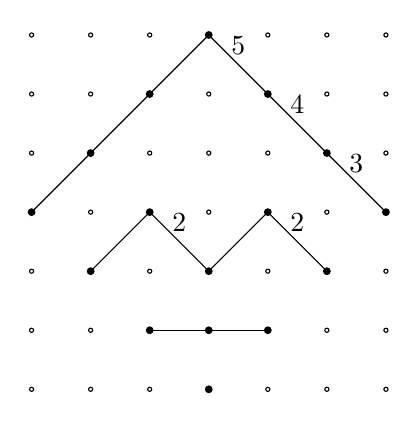
\begin{tikzpicture}[scale=0.75]
\foreach \i in {0,...,6}
	\foreach \j in {0,...,6}{
		\draw (\i,\j) circle(1pt);
	};
	
	% 0 level
	\node at (3,0) [circle, fill, inner sep=1pt]{};
	
	% 1 level
	\node at (2,1) [circle, fill, inner sep=1pt]{};
	\node at (3,1) [circle, fill, inner sep=1pt]{};
	\node at (4,1) [circle, fill, inner sep=1pt]{};
	\draw (2,1) -- (4,1);
	
	% 2 level
	\node at (1,2) [circle, fill, inner sep=1pt]{};
	\node at (2,3) [circle, fill, inner sep=1pt]{};
	\node at (3,2) [circle, fill, inner sep=1pt]{};
	\node at (4,3) [circle, fill, inner sep=1pt]{};
	\node at (5,2) [circle, fill, inner sep=1pt]{};
	\draw (1,2) -- (2,3);
	\draw (2,3) -- node[above] {2} (3,2);
	\draw (3,2) -- (4,3);
	\draw (4,3) -- node[above] {2} (5,2);
	
	% 3 level
	\node at (0,3) [circle, fill, inner sep=1pt]{};
	\node at (1,4) [circle, fill, inner sep=1pt]{};
	\node at (2,5) [circle, fill, inner sep=1pt]{};
	\node at (3,6) [circle, fill, inner sep=1pt]{};
	\node at (4,5) [circle, fill, inner sep=1pt]{};
	\node at (5,4) [circle, fill, inner sep=1pt]{};
	\node at (6,3) [circle, fill, inner sep=1pt]{};
	\draw (0,3) -- (1,4) -- (2,5) -- (3,6);
	\draw (3,6) -- node[above] {5} (4,5);
	\draw (4,5) -- node[above] {4} (5,4);
	\draw (5,4) -- node[above] {3} (6,3);
\end{tikzpicture}
\end{equation*}
\caption{\label{fig:Mpath} A disjoint 3-collection containing a flat step at height 1 and an M-path at height 2 with $\omega_2$ weightings.}
\end{figure}

Since we can recognize $X_{m-1}^1$ as a union of disjoint $(m-1)$-collections with this specific form, we can write down an explicit expression for $D'$:
\begin{equation*}
D' = \sum\limits_{\substack{1\leq p\leq m-1\\0\leq q\leq m-1-p}}\left(\prod\limits_{k=0}^{p-1}\frac{(2k+1)!}{(k+1)!}\right)\left(\frac{(2p)!}{(p+1)!}\right)\left(\prod\limits_{k=p+1}^{p+q}\frac{(2k)!(2k)}{(k+1)!}\right)\left(\prod\limits_{k=p+q+1}^{m-1}\frac{(2k+1)!}{(k+1)!}\right).
\end{equation*}

We can simplify the quotient $D'/D$: For each summand depending on $p,q$ in the quotient $D'/D$, we have
\begin{equation*}
\frac{\prod\limits_{k=0}^{p-1}\frac{1}{(k+1)!}\frac{1}{p!}\prod\limits_{k=p+1}^{p+q}\frac{1}{(k+1)!}\prod\limits_{k=p+q+1}^{m-1}\frac{1}{(k+1)!}\prod\limits_{k=0}^{p-1}(2k+1)!(2p)!\prod\limits_{k=p+1}^{p+q}(2k)!(2k)\prod\limits_{k=p+q+1}^{m-1}(2k+1)!}{\prod\limits_{k=0}^{m-1}\frac{1}{(k+1)!}\prod\limits_{k=0}^{m-1}(2k+1)!}.
\end{equation*}
We can cancel the product of all the $\frac{1}{(k+1)!}$'s since on the top we also have a product of $\frac{1}{(k+1)!}$'s from 0 up to $m-1$. This gives us
\begin{equation*}
\frac{\prod\limits_{k=0}^{p-1}(2k+1)!(2p)!\prod\limits_{k=p+1}^{p+q}(2k)!(2k)\prod\limits_{k=p+q+1}^{m-1}(2k+1)!}{\prod\limits_{k=0}^{m-1}(2k+1)!}.
\end{equation*}
We can further cancel all the $(2k+1)!$'s from $k = 0$ to $p-1$ and from $p+q+1$ to $m-1$:
\begin{align*}
\frac{(2p)!\prod\limits_{k=p+1}^{p+q}(2k)!(2k)}{\prod\limits_{k=p}^{p+q}(2k+1)!} &= \frac{(2p)!\prod\limits_{k=p+1}^{p+q}(2k)!(2k)}{(2p+1)!\prod\limits_{k=p+1}^{p+q}(2k+1)! }\\
&=\frac{1}{2p+1}\left(\prod\limits_{k=p+1}^{p+q}\frac{2k}{2k+1}\right). \\
\end{align*}
So summing over all such $p$ and $q$ we have
\begin{equation}\label{eqn:D'/D}
\frac{D'}{D} = \sum\limits_{\substack{1\leq p \leq m-1 \\ 0 \leq q \leq m - 1 - p}}\frac{1}{2p+1}\prod\limits_{k=p+1}^{p+q}\left(\frac{2k}{2k+1}\right).
\end{equation}

\section{Disjoint $k$-collections with two flat steps}

Recall for $N''$ and $D''$ (equations (\ref{eqn:N''}) and (\ref{eqn:D''}) above) we are considering paths in disjoint $k$-collections from either $X_{m+1}^2$ or $X_{m-1}^2$. So our next step is to describe all disjoint $k$-collections containing exactly two flat steps. We can already rule out the possibility where a disjoint $k$-collection has two flat steps on the same path. This is because any path below the one with the flat steps needs to be a V-path and there's then not enough room on the path with the flat step for a flat step to appear anywhere other than the center. This then also tells us that for any disjoint $k$-collection with two flat steps, the two flat steps will be on separate paths and moreover the first flat step will be centered.

As before, after the first flat step we can have some number of M-paths followed by some number of V-paths. If we have a nonzero amount of V-paths, then that means the second path with a flat step in it will have its flat step centered. On the other hand, if we only have M-paths above the first flat step path, then we have enough room for the second path containing a flat step to have its flat step offset by one either to the left or right, that is, either a path starting at height $k$ with $(k-2)$ ascents, followed by a flat step, one more ascent and then $(k-1)$ descents, or a path starting at height $k$ with $(k-1)$ ascents, one descent, a flat step and then $(k-2)$ descents. Notice that by symmetry, a path with flat step offset to the left has same total weight as a path with flat step offset to the right, and moreover that both have a total weight  equal to the total weight of a regular flat step path at the same height. For this reason, in the future when discussing the total weight, we will use the term ``flat step path'' to refer to both types of paths. Suppose we have a left-offset flat step path at height $p$, then on the path at height $p+1$ we have enough space to have a left \textbf{asymmetric M-path} consisting of $(p+1-2)$ ascents, followed by one descent, 2 ascents, and then $(p+1-1)$ descents. More generally, a (left) asymmetric M-path at height $k$ consists of $(k-2)$ ascents, one descent, two ascents and then $(k-1)$ descents. Above this first left asymmetric M-path we can have more asymmetric M-paths or regular M-paths or V-paths.

Suppose we have an left asymmetric M-path $\sigma$ at height $k$, then the product of the weights on this path is given by
\begin{equation*}
\omega_2(\sigma) = \frac{(2k-2)!}{(k-1)!}(2k-3).
\end{equation*}
Notice that by symmetry, a right asymmetric M-path (corresponding to the case where the second flat step is off-set to the right) will have the same product of weights. This means that a disjoint $k$-collection of where the second flat step is offset to the left followed by left asymmetric M-paths will have the same total weighting as the disjoint $k$-collection yielded by reflecting across the $y$-axis. For this reason, we will only need to consider the left offset case.

To summarize, we have two cases of disjoint $k$-collections containing exactly two flat steps:
\begin{enumerate}[label=(\alph*)]
\item Two centred flat steps: We have two centered flat step paths at height $p_1$ and $p_2$ respectively. Above the first flat step path we have $q_1$ M-paths and above the second flat step path we have $q_2$ M-paths. V-paths fill in all the rest. We will denote these kinds of disjoint $k$-collections by $\sigma_{p_1,p_2,q_1,q_2}^k$.
\item Second flat step is offset: We have one centered flat step path at height $p_1$ and an offset flat step path at height $p_2$. In between $p_1$ and $p_2$ we have only M-paths. Above the second flat step path we have $q_1$ asymmetric M-paths followed by $q_2$ M-paths. V-paths fill in the top and the bottom. We will denote disjoint $k$-collections of this form by $L_{p_1,p_2,q_1,q_2}^k$ for a left offset and $R_{p_1,p_2,q_1,q_2}^k$ for a right offset (though as remarked above, we will only need to consider the left offset case).
\end{enumerate}

So we have that
\begin{equation*}
X_{k}^2 = \bigcup\limits_{p_1,p_2,q_1,q_2}\sigma_{p_1,p_2,q_1,q_2}^k \cup \bigcup\limits_{p_1,p_2,q_1,q_2}L_{p_1,p_2,q_1,q_2}^k \cup \bigcup\limits_{p_1,p_2,q_1,q_2}R_{p_1,p_2,q_1,q_2}^k.
\end{equation*}

\begin{figure}
\begin{equation*}
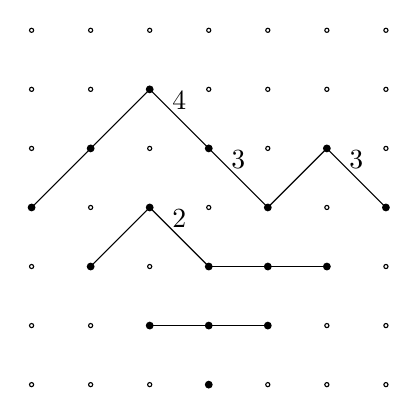
\begin{tikzpicture}[scale=0.75]
\foreach \i in {0,...,6}
	\foreach \j in {0,...,6}{
		\draw (\i,\j) circle(1pt);
	};
	
	% 0 level
	\node at (3,0) [circle, fill, inner sep=1pt]{};
	
	% 1 level
	\node at (2,1) [circle, fill, inner sep=1pt]{};
	\node at (3,1) [circle, fill, inner sep=1pt]{};
	\node at (4,1) [circle, fill, inner sep=1pt]{};
	\draw (2,1) -- (4,1);
	
	% 2 level
	\node at (1,2) [circle, fill, inner sep=1pt]{};
	\node at (2,3) [circle, fill, inner sep=1pt]{};
	\node at (3,2) [circle, fill, inner sep=1pt]{};
	\node at (4,2) [circle, fill, inner sep=1pt]{};
	\node at (5,2) [circle, fill, inner sep=1pt]{};
	\draw (1,2) -- (2,3);
	\draw (2,3) -- node[above] {2} (3,2);
	\draw (3,2) -- (4,2) -- (5,2);
	
	% 3 level
	\node at (0,3) [circle, fill, inner sep=1pt]{};
	\node at (1,4) [circle, fill, inner sep=1pt]{};
	\node at (2,5) [circle, fill, inner sep=1pt]{};
	\node at (3,4) [circle, fill, inner sep=1pt]{};
	\node at (4,3) [circle, fill, inner sep=1pt]{};
	\node at (5,4) [circle, fill, inner sep=1pt]{};
	\node at (6,3) [circle, fill, inner sep=1pt]{};
	\draw (0,3) -- (1,4) -- (2,5);
	\draw (2,5) -- node[above] {4} (3,4);
	\draw (3,4) -- node[above] {3} (4,3);
	\draw (4,3) -- (5,4);
	\draw (5,4) -- node[above] {3} (6,3);
\end{tikzpicture}
\end{equation*}
\caption{\label{fig:asymMpath} A disjoint 3-collection containing two flat steps (one off-centered) and an asymmetric M-path with $\omega_2$ weightings.}
\end{figure}

\subsection{$\mu$ Simplification of the $N''-d!D''$ Term}

Recall that for $N''$ and $D''$ we have:
\begin{equation*}
N'' = t^{-2}\sum\limits_{\sigma\in X_{m+1}^2}\prod\limits_{\tau\in\sigma}\omega_2(\tau),\quad D'' = t^{-2}\sum\limits_{\sigma\in X_{m-1}^2}\prod\limits_{\tau\in\sigma}\omega_0(\tau),
\end{equation*}
so in $N''$ we are considering disjoint $(m+1)$-collections with exactly two flat steps while in $D''$ we are considering disjoint $(m-1)$-collections. In order to not have to consider both, we employ the same trick originally used in \cite{willerton_magnitude_2017} to show $N = d!D$ (which we will call $\mu$ simplification). The idea is to view disjoint $(m-1)$-collections in $X_{m-1}$ as being embedded in $X_{m+1}$ and so we only need to work in $X_{m+1}^2$. Let $\sigma \in X_{m-1}$, then we get a corresponding $\mu(\sigma)\in X_{m+1}$ by shifting all paths up two units, adding ascents from $(-i,i)$ to $(-i+1,i+1)$ and descents from $(i-1,i+1)$ to $(i,i)$ for $1\leq i \leq m$, and finally adding a V-path at height $m+1$. Then $\mu(\sigma)$ has the same number of flat steps as $\sigma$ and
\begin{equation}\label{eqn:mu}
\prod\limits_{\tau\in\mu(\sigma)}\omega_2(\tau) = d!\prod\limits_{\tau\in\sigma}\omega_0(\tau).
\end{equation}
Let $\mu(X_{m-1}^2)\subseteq X_{m+1}^2$ denote the disjoint $(m+1)$-collections that are these embeddings of all the disjoint $(m-1)$-collections in $X_{m-1}^2$, then by (\ref{eqn:mu}), we have
\begin{align*}
N''-d!D'' &= t^{-2}\sum\limits_{\sigma\in X_{m+1}^2}\prod\limits_{\tau\in\sigma}\omega_2(\tau) - d!t^{-2}\sum\limits_{\sigma\in X_{m-1}^2}\prod\limits_{\tau\in\sigma}\omega_0(\tau) \\
&= t^{-2}\sum\limits_{\sigma\in X_{m+1}^2\setminus\mu(X_{m-1}^2)}\prod\limits_{\tau\in\sigma}\omega_2(\tau).
\end{align*}
So our next step is to describe all disjoint $(m+1)$-collections with two flat steps that are not embeddings of disjoint $(m-1)$-collections with two flat steps. We have four disjoint cases:
\begin{enumerate}
\item The first flat step at height $p_1=1$ and the second flat step is at height $p_2$ where $2\leq p_2\leq m+1$.
\item The first flat step is at height $p_1 \geq 2$. The second flat step is at height $p_2 = m$ and we either have a M-path or an asymmetric M-path above $p_2$.
\item The first flat step is at height $p_1 \geq 2$. The second flat step is at height $p_2 = m+1$.
\item The two flat steps are at heights between $2$ and $m-1$ but with no V-paths above height $p_2$.
\end{enumerate}
Abusing notation slightly, let $\sigma$ be the total weighting of the disjoint collections that are in any of the four cases above and moreover have two centered flat steps. Let $L$ be the corresponding weighting for disjoint collections where the second flat step is offset to the left and let $R$ be the corresponding weighting where the second flat step is offset to the right. By the symmetry reasoning above, we have that $L=R$, so we have that
\begin{equation}\label{eqn:L=R}
N'' - d!D'' = \sigma + L + R = \sigma + 2L
\end{equation}
We explicitly give expressions for $\sigma$ and $L$ below:
\begin{equation}\label{eqn:sigma}
\begin{aligned}
\sigma = &\sum\limits_{\substack{2\leq p_2\leq m+1 \\ 0\leq q_1 \leq p_2-2 \\ 0 \leq q_2 \leq m+1-p_2}}\omega_2(\sigma_{1,p_2,q_1,q_2}^{m+1}) + \sum\limits_{\substack{2 \leq p_1 \leq m-1 \\ 0 \leq q_1 \leq m-p_1-1}}\omega_2(\sigma_{p_1,m,q_1,m+1-p_2}^{m+1}) \\
 &\quad+ \sum\limits_{\substack{2 \leq p_1 \leq m \\ 0 \leq q_1 \leq m-p_1}}\omega_2(\sigma_{p_1,m+1,q_1,0}^{m+1}) + \sum\limits_{\substack{2 \leq p_1 \leq m \\ p_1+1 \leq p_2 \leq m-1 \\ 0 \leq q_1 \leq p_2-p_1-1}} \omega_2(\sigma_{p_1,p_2,q_1,m+1-p_2}^{m+1})
\end{aligned}
\end{equation}
and
\begin{equation}\label{eqn:L}
\begin{aligned}
L = &\sum\limits_{\substack{2\leq p_2\leq m+1 \\ 0\leq q_1 \leq p_2-2 \\ 0 \leq q_2 \leq m+1-p_2}}\omega_2(L_{1,p_2,q_1,q_2}^{m+1}) + \sum\limits_{\substack{2 \leq p_1 \leq m-1 \\ 0 \leq q_1 \leq m-p_1-1}}\omega_2(L_{p_1,m,q_1,m+1-p_2}^{m+1}) \\
 &\quad+ \sum\limits_{\substack{2 \leq p_1 \leq m \\ 0 \leq q_1 \leq m-p_1}}\omega_2(L_{p_1,m+1,q_1,0}^{m+1}) + \sum\limits_{\substack{2 \leq p_1 \leq m \\ p_1+1 \leq p_2 \leq m-1 \\ 0 \leq q_1 \leq p_2-p_1-1}} \omega_2(L_{p_1,p_2,q_1,m+1-p_2}^{m+1}).
\end{aligned}
\end{equation}

\subsection{Proof that $\sigma = L$}

It might seem overwhelming to have to calculate both $\sigma$ and $L$, however, the following lemma allows us to bypass one of these calculations.

\begin{lem}\label{lem:sigma=L}
Let $\sigma$ and $L$ be given respectively as in (\ref{eqn:sigma}) and (\ref{eqn:L}) above. Then $\sigma = L$. 
\end{lem}

\begin{proof}
We prove the lemma by showing that there is a bijection of sets $f:\sigma \to L$ that preserves the product of the weights in each disjoint $(m+1)$-collection. Let $\delta$ be a disjoint $(m+1)$-collection in $\sigma$. In general, $\delta$ will have its first flat step at $p_1$ and second flat step at $p_2$. In between the two flat steps there will be $q_1$ M-paths followed by $p_2-p_1-q_1$ number of V-paths. We'll call the height at which this first V-path appears to be $v$. Then we define $f(\delta)$ to be a disjoint $(m+1)$-collection in $L$ where we take $\delta$ and replace the V-path at $v$ with a off-centred flat step path and all the paths from $v+1$ up to $p_2$ are replaced with asymmetric M-paths. If $\delta$ had no V-paths in between the first two flat steps, then just replace the second flat step with an off-centred flat step. Clearly $f(\delta)$ is a unique disjoint $(m+1)$-collection in $L$ and this defines a well-defined function of sets from $\sigma$ to $L$. We can see that $f$ preserves the product of the weights on $\delta$: each V-path starting at a height of say, $h$ had product of weights $\frac{(2h-1)!}{(h-1)!}$ and this path was replaced by an asymmetric M-path with product of weights $\frac{(2h-2)!}{(h-1)!}$ but on the asymmetric M-path of height $h+1$ we have an extra factor of $(2(h+1)-3) = (2h+2-3) = (2h-1)$ so in total we also have product of weights $\frac{(2h-1)!}{(h-1)!}$. Note that this also applies to the flat step we introduced at height $v$: it had product of weights $\frac{(2v-2)!}{(v-1)!}$ but the asymmetric M-path just above it gives an extra factor of $(2v-1)$ which is already accounted for. Finally the flat step at $p_2$ in $\delta$ had product of weights $\frac{(2p_2-2)!}{(p_2-1)}$ which is the same as the product of the weights in the asymmetric M-path we introduced at $p_2$. So we see that $f$ preserves weighting. An example of two disjoint collections with the same product of weights that are identified by $f$ is given in Figure \ref{fig:43200} below.

Now we define a function $g:L\to\sigma$. Let $\delta$ instead be a disjoint $(m+1)$-collection in $L$. The collection $\delta$ has a second off-centred flat step at height $p_2$ with $q_1$ number of asymmetric M-paths above it. Then we define $g(\delta)$ to be the disjoint $(m+1)$-collection where we replace the second flat step at $p_2$ and all the asymmetric M-paths above it with V-paths except for the last one, which we turn into a centred flat step (ie. at height $p_2+q_1$. The paths above $p_2+q_1$ will be either V-paths or (symmetric) M-paths and so this gives us a disjoint $(m+1)$-collection in $\sigma$. Clearly, $g,f$ are inverse to each other, giving us a bijection $\sigma\to L$. Since $f$ preserves products of weights, this also gives us that $\sigma = L$ as values.
\end{proof}

\begin{figure}[h!]
\begin{equation*}
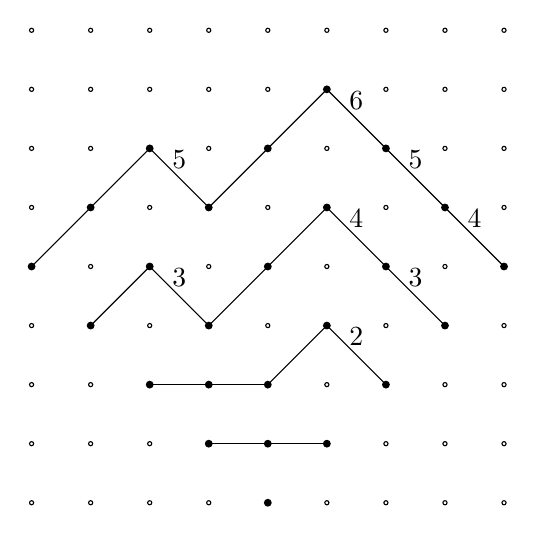
\begin{tikzpicture}[scale=0.75]
\foreach \i in {0,...,8}
	\foreach \j in {0,...,8}{
		\draw (\i,\j) circle(1pt);
	};
	
	% 0 level
	\node at (4,0) [circle, fill, inner sep=1pt]{};
	
	% 1 level
	\node at (3,1) [circle, fill, inner sep=1pt]{};
	\node at (4,1) [circle, fill, inner sep=1pt]{};
	\node at (5,1) [circle, fill, inner sep=1pt]{};
	\draw (3,1) -- (5,1);
	
	% 2 level
	\node at (2,2) [circle, fill, inner sep=1pt]{};
	\node at (3,2) [circle, fill, inner sep=1pt]{};
	\node at (4,2) [circle, fill, inner sep=1pt]{};
	\node at (5,3) [circle, fill, inner sep=1pt]{};
	\node at (6,2) [circle, fill, inner sep=1pt]{};
	\draw (2,2) -- (3,2) -- (4,2);
	\draw (4,2) -- (5,3);
	\draw (5,3) -- node[above] {2} (6,2);
	
	% 3 level
	\node at (1,3) [circle, fill, inner sep=1pt]{};
	\node at (2,4) [circle, fill, inner sep=1pt]{};
	\node at (3,3) [circle, fill, inner sep=1pt]{};
	\node at (4,4) [circle, fill, inner sep=1pt]{};
	\node at (5,5) [circle, fill, inner sep=1pt]{};
	\node at (6,4) [circle, fill, inner sep=1pt]{};
	\node at (7,3) [circle, fill, inner sep=1pt]{};
	\draw (1,3) -- (2,4);
	\draw (2,4) -- node[above] {3} (3,3);
	\draw (3,3) -- (4,4) -- (5,5);
	\draw (5,5) -- node[above] {4} (6,4);
	\draw (6,4) -- node[above] {3} (7,3);
	
	% 4 level
	\node at (0,4) [circle, fill, inner sep=1pt]{};
	\node at (1,5) [circle, fill, inner sep=1pt]{};
	\node at (2,6) [circle, fill, inner sep=1pt]{};
	\node at (3,5) [circle, fill, inner sep=1pt]{};
	\node at (4,6) [circle, fill, inner sep=1pt]{};
	\node at (5,7) [circle, fill, inner sep=1pt]{};
	\node at (6,6) [circle, fill, inner sep=1pt]{};
	\node at (7,5) [circle, fill, inner sep=1pt]{};
	\node at (8,4) [circle, fill, inner sep=1pt]{};
	\draw (0,4) -- (1,5) -- (2,6);
	\draw (2,6) -- node[above] {5} (3,5);
	\draw (3,5) -- (4,6) -- (5,7);
	\draw (5,7) -- node[above] {6} (6,6);
	\draw (6,6) -- node[above] {5} (7,5);
	\draw (7,5) -- node[above] {4} (8,4);

\end{tikzpicture}\qquad
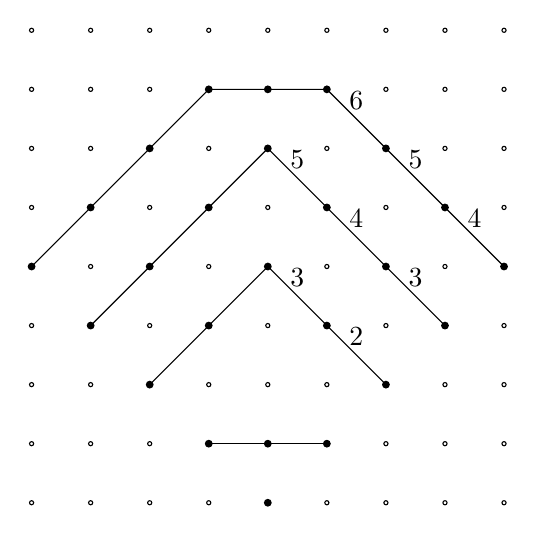
\begin{tikzpicture}[scale=0.75]
\foreach \i in {0,...,8}
	\foreach \j in {0,...,8}{
		\draw (\i,\j) circle(1pt);
	};
	
	% 0 level
	\node at (4,0) [circle, fill, inner sep=1pt]{};
	
	% 1 level
	\node at (3,1) [circle, fill, inner sep=1pt]{};
	\node at (4,1) [circle, fill, inner sep=1pt]{};
	\node at (5,1) [circle, fill, inner sep=1pt]{};
	\draw (3,1) -- (5,1);
	
	% 2 level
	\node at (2,2) [circle, fill, inner sep=1pt]{};
	\node at (3,3) [circle, fill, inner sep=1pt]{};
	\node at (4,4) [circle, fill, inner sep=1pt]{};
	\node at (5,3) [circle, fill, inner sep=1pt]{};
	\node at (6,2) [circle, fill, inner sep=1pt]{};
	\draw (2,2) -- (3,3) -- (4,4);
	\draw (4,4) -- node[above] {3} (5,3);
	\draw (5,3) -- node[above] {2} (6,2);
	
	% 3 level
	\node at (1,3) [circle, fill, inner sep=1pt]{};
	\node at (2,4) [circle, fill, inner sep=1pt]{};
	\node at (3,5) [circle, fill, inner sep=1pt]{};
	\node at (4,6) [circle, fill, inner sep=1pt]{};
	\node at (5,5) [circle, fill, inner sep=1pt]{};
	\node at (6,4) [circle, fill, inner sep=1pt]{};
	\node at (7,3) [circle, fill, inner sep=1pt]{};
	\draw (1,3) -- (2,4) -- (3,5) -- (4,6);
	\draw (4,6) -- node[above] {5} (5,5);
	\draw (5,5) -- node[above] {4} (6,4);
	\draw (6,4) -- node[above] {3} (7,3);
	
	% 4 level
	\node at (0,4) [circle, fill, inner sep=1pt]{};
	\node at (1,5) [circle, fill, inner sep=1pt]{};
	\node at (2,6) [circle, fill, inner sep=1pt]{};
	\node at (3,7) [circle, fill, inner sep=1pt]{};
	\node at (4,7) [circle, fill, inner sep=1pt]{};
	\node at (5,7) [circle, fill, inner sep=1pt]{};
	\node at (6,6) [circle, fill, inner sep=1pt]{};
	\node at (7,5) [circle, fill, inner sep=1pt]{};
	\node at (8,4) [circle, fill, inner sep=1pt]{};
	\draw (0,4) -- (1,5) -- (2,6) -- (3,7) -- (4,7) -- (5,7);
	\draw (5,7) -- node[above] {6} (6,6);
	\draw (6,6) -- node[above] {5} (7,5);
	\draw (7,5) -- node[above] {4} (8,4);

\end{tikzpicture}
\end{equation*}
\caption{\label{fig:43200} Two corresponding disjoint $4$-collections under the bijection $f$. The total product of weights if 43200 for both collections.}
\end{figure}

\subsection{Simplifying the $\sigma$ Term}

Since we understand V-paths, we can immediately write down an explicit expression for $N$:
\begin{equation*}
N = \prod\limits_{\tau\in\sigma_{\text{roof}}^{m+1}}\omega_2(\tau) = \prod\limits_{k=1}^{m+1}\frac{(2k-1)!}{(k-1)!}.
\end{equation*}

So by the equality of $\sigma$ and $L$ and (\ref{eqn:L=R}), we have
\begin{equation*}
\frac{N''-d!D''}{N} = \frac{\sigma + 2L}{N} = \frac{3\sigma}{N}.
\end{equation*}

Earlier we had split $\sigma$ into four smaller sums based on which case they fell into (equation (\ref{eqn:sigma})). Consider a disjoint $(m+1)$-collection in the first case, that is, we fix $p_1 = 1$, $2\leq p_2\leq m+1$, $0\leq q_1\leq p_2 - 2$, $0\leq q_2 \leq m+1-p_2$. Then each summand in this first sum is given by
\begin{align*}
\frac{\sigma'}{N} &= \frac{\left(\prod\limits_{k=2}^{q_1+2}(2k-2)!(2k-2)\right)\left(\prod\limits_{k=q_1+2}^{p_2-1}(2k-1)!\right)(2p_2-2)!\left(\prod\limits_{k=p_2+1}^{p_2+q_2}(2k-2)!(2k-2)\right)\left(\prod\limits_{k=p_2+q_2+1}^{m+1}(2k-1)!\right)}{\left(\prod\limits_{k=0}^{m+1}(2k-1)!\right)} \\
&= \frac{\left(\prod\limits_{k=2}^{q_1+2}(2k-2)!(2k-2)\right)(2p_2-2)!\left(\prod\limits_{k=p_2+1}^{p_2+q_2}(2k-2)!(2k-2)\right)}{\left(\prod\limits_{k=2}^{q_1+2}(2k-1)!\right)\left(\prod\limits_{k=p_2}^{p_2+q_2}(2k-1)!\right)} \\
&= \frac{1}{2p_2-1}\left(\prod\limits_{k=2}^{q_1+2}\frac{(2k-2)}{(2k-1)}\right)\left(\prod\limits_{k=p_2+1}^{p_2+q_2}\frac{(2k-2)}{(2k-1)}\right).
\end{align*}

So for the first case, we have
\begin{equation}\label{eqn:sigma1}
\frac{\sigma_1}{N} = \sum\limits_{\substack{2\leq p_2\leq m+1 \\ 0\leq q_1 \leq p_2-2 \\ 0\leq q_2 \leq m+1-p_2}}\frac{1}{2p_2-1}\left(\prod\limits_{k=2}^{q_1+2}\frac{(2k-2)}{(2k-1)}\right)\left(\prod\limits_{k=p_2+1}^{p_2+q_2}\frac{(2k-2)}{(2k-1)}\right).
\end{equation}

We similarly find expressions for the other three smaller sums.

Consider a disjoint $(m+1)$-collection in the second case, that is, we fix $2\leq p_1\leq m-1$,$p_2=m$,$0\leq q_1\leq m-p_1-1$, $q_2 = 1$. Then each summand is given by
\begin{equation*}
\frac{\sigma'}{N} = \frac{1}{2p_1-1}\left(\prod\limits_{k=p_1+1}^{p_1+q_1}\frac{(2k-2)}{(2k-1)}\right)\left(\frac{2m}{(2m-1)(2m+1)}\right)
\end{equation*}
and for the second case, we have
\begin{equation}\label{eqn:sigma2}
\frac{\sigma_2}{N} = \sum\limits_{\substack{2\leq p_1\leq m-1 \\ 0\leq q_1\leq m-p_1-1}}\frac{1}{2p_1-1}\left(\prod\limits_{k=p_1+1}^{p_1+q_1}\frac{(2k-2)}{(2k-1)}\right)\left(\frac{2m}{(2m-1)(2m+1)}\right).
\end{equation}

Consider a disjoint $(m+1)$-collection in the third case. Then each summand is given by
\begin{equation*}
\frac{\sigma'}{N} = \frac{1}{2p_1-1}\left(\prod\limits_{k=p_1+1}^{p_1+q_1}\frac{(2k-2)}{(2k-1)}\right)\left(\frac{1}{2m+1}\right)
\end{equation*}
and for the third case, we have
\begin{equation}\label{eqn:sigma3}
\frac{\sigma_3}{N} = \sum\limits_{\substack{2\leq p_1\leq m \\ 0\leq q_1\leq m-p_1}}\frac{1}{2p_1-1}\left(\prod\limits_{k=p_1+1}^{p_1+q_1}\frac{(2k-2)}{(2k-1)}\right)\left(\frac{1}{2m+1}\right).
\end{equation}

Consider a disjoint $(m+1)$-collection in the fourth case. Then each summand is given by
\begin{equation*}
\frac{\sigma'}{N} = \frac{1}{2p_1-1}\left(\prod\limits_{k=p_1+1}^{p_1+q_1}\frac{(2k-2)}{(2k-1)}\right)\frac{1}{2p_2-1}\left(\prod\limits_{k=p_2+1}^{m+1}\frac{(2k-2)}{(2k-1)}\right)
\end{equation*}
and for the fourth case, we have
\begin{equation}\label{eqn:sigma4}
\frac{\sigma_4}{N} = \sum\limits_{\substack{2\leq p_1\leq m \\ p_1+1\leq p_2 \leq m-1 \\ 0\leq q_1\leq p_2-p_1-1 }}\frac{1}{2p_1-1}\left(\prod\limits_{k=p_1+1}^{p_1+q_1}\frac{(2k-2)}{(2k-1)}\right)\frac{1}{2p_2-1}\left(\prod\limits_{k=p_2+1}^{m+1}\frac{(2k-2)}{(2k-1)}\right).
\end{equation}

\subsection{Putting It All Together}

So combining (\ref{eqn:D'/D}), (\ref{eqn:sigma1}), (\ref{eqn:sigma2}), (\ref{eqn:sigma3}) and (\ref{eqn:sigma4}) together, we give an explicit expression for
\begin{equation*}
\frac{d^2}{dt^2}\text{Mag}\left(tB_2^d\right).
\end{equation*}

\begin{theo}\label{theo:partialres}
Let $d$ be odd and $B_2^d$ be the closed $d$-dimensional Euclidean ball. Then
\begin{equation}
\begin{aligned}
&\frac{d^2}{dt^2}\text{Mag}(tB_2^d)\big\vert_{t=0} = \\
&6\sum\limits_{\substack{2\leq p_2\leq m+1 \\ 0\leq q_1 \leq p_2-2 \\ 0\leq q_2 \leq m+1-p_2}}\frac{1}{2p_2-1}\left(\prod\limits_{k=2}^{q_1+2}\frac{(2k-2)}{(2k-1)}\right)\left(\prod\limits_{k=p_2+1}^{p_2+q_2}\frac{(2k-2)}{(2k-1)}\right) + \\
&6\sum\limits_{\substack{2\leq p_1\leq m-1 \\ 0\leq q_1\leq m-p_1-1}}\frac{1}{2p_1-1}\left(\prod\limits_{k=p_1+1}^{p_1+q_1}\frac{(2k-2)}{(2k-1)}\right)\left(\frac{2m}{(2m-1)(2m+1)}\right) + \\
&6\sum\limits_{\substack{2\leq p_1\leq m \\ 0\leq q_1\leq m-p_1}}\frac{1}{2p_1-1}\left(\prod\limits_{k=p_1+1}^{p_1+q_1}\frac{(2k-2)}{(2k-1)}\right)\left(\frac{1}{2m+1}\right) + \\
&6\sum\limits_{\substack{2\leq p_1\leq m \\ p_1+1\leq p_2 \leq m-1 \\ 0\leq q_1\leq p_2-p_1-1 }}\frac{1}{2p_1-1}\left(\prod\limits_{k=p_1+1}^{p_1+q_1}\frac{(2k-2)}{(2k-1)}\right)\frac{1}{2p_2-1}\left(\prod\limits_{k=p_2+1}^{m+1}\frac{(2k-2)}{(2k-1)}\right) - \\
&V_{1}\sum\limits_{\substack{1\leq p \leq m-1 \\ 0 \leq q \leq m - 1 - p}}\frac{1}{2p+1}\prod\limits_{k=p+1}^{p+q}\left(\frac{2k}{2k+1}\right).
\end{aligned}
\end{equation}
\end{theo}

%\subsection{Skip Factorials}
%
%The products
%\begin{equation*}
%\prod\limits_{k=a}^{b}\frac{(2k-2)}{(2k-1)},\qquad\prod\limits_{k=a}^b\frac{2k}{2k+1}
%\end{equation*}
%that appear in the sums above are ratios of skip or double factorials. In the following, we will refer to the identities about skip factorials given just below:
%\begin{align*}
%&(2n)!! = 2^nn! \\
%&(2n-1)!! = \frac{(2n)!}{2^nn!} \\
%&(2n+1)!! = \frac{(2n+1)!}{2^nn!}
%\end{align*}
%We will also use Catalan numbers, which are defined by
%\begin{equation*}
%C_n = \frac{1}{n+1}\binom{(2n)}{n} = \frac{1}{2n+1}\binom{(2n+1)}{n}
%\end{equation*}
%Now let's write the product
%\begin{equation*}
%\prod\limits_{k=a}^{b}\frac{(2k-2)}{(2k-1)}
%\end{equation*}
%in terms of skip factorials and try to simplify from there:
%\begin{align*}
%\prod\limits_{k=a}^{b}\frac{(2k-2)}{(2k-1)} &= \frac{2(a-1)}{2a-1}\cdots\frac{2(b-1)}{2b-1} \\
%&= \frac{(2(b-1))!!}{(2(a-2))!!}\left[\frac{(2b-1)!!}{(2(a-1)-1)!!}\right]^{-1} \\
%&= \frac{2^{b-1}(b-1)!}{2^{a-2}(a-2)!}\left[\frac{(2b)!}{2^bb!}\frac{2^{a-1}(a-1)!}{(2(a-1))!}\right]^{-1} \\
%&= \frac{2^{2b-1}}{2^{2(a-1)-1}}\frac{b!(b-1)!}{(2b)!}\frac{(2(a-1))!}{(a-1)!(a-2)!} \\
%&= \frac{2^{2b-1}}{2^{2(a-1)-1}}\frac{(a-1)\binom{2(a-1)}{a-1}}{b\binom{2b}{b}} \\
%&= \frac{2^{2b-1}}{2^{2(a-1)-1}}\frac{(a-1)aC_{a-1}}{b(b+1)C_b}
%\end{align*}
%And similarly:
%\begin{align*}
%\prod\limits_{k=a}^b\frac{2k}{2k+1} &= \frac{2a}{2a+1}\cdots\frac{2b}{2b+1} \\
%&= \frac{(2b)!!}{(2(a-1))!!}\left[\frac{(2b+1)!!}{(2a-1)!!}\right]^{-1} \\
%&= \frac{2^bb!}{2^{a-1}(a-1)!}\left[\frac{(2b+1)!}{2^bb!}\frac{2^aa!}{(2a)!}\right]^{-1} \\
%&= \frac{2^{2b}}{2^{2a-1}}\frac{(b!)^2}{(2b+1)!}\frac{(2a)!}{a!(a-1)!} \\
%&= \frac{2^{2b}}{2^{2a-1}}\frac{a\binom{2a}{a}}{(b+1)\binom{2b+1}{b}} \\
%&= \frac{2^{2b}}{2^{2a-1}}\frac{a(a+1)C_a}{(2b+1)(b+1)C_b}
%\end{align*}
%
%Using the above, we can rewrite the last sum in our expression for the second derivative as the following:
%\begin{equation*}
%V_{1}\sum\limits_{\substack{1\leq p \leq m-1 \\ 0 \leq q \leq m - 1 - p}}\frac{1}{2p+1}\prod\limits_{k=p+1}^{p+q}\left(\frac{2k}{2k+1}\right) = V_1\sum\limits_{\substack{1\leq p \leq m-1 \\ 0 \leq q \leq m-1}} \frac{1}{2p+1}\frac{2^{2(p+q)}}{2^{2(p+1)-1}}\frac{(p+1)(p+2)C_{p+1}}{(2(p+q)+1)(p+q+1)C_{p+q}}
%\end{equation*}
%Setting $k = p+q$, this last sum turns into
%\begin{align*}
%&V_1\sum\limits_{k=1}^{m-1}\sum\limits_{p=1}^k\frac{1}{2p+1}\frac{2^{2k}}{2^{2(p+1)-1}}\frac{(p+1)(p+2)C_{p+1}}{(2k+1)(k+1)C_k} = V_1\sum\limits_{k=1}^{m-1}\frac{2^{2k}}{(2k+1)(k+1)C_k}\sum\limits_{p=1}^k\frac{(p+1)(p+2)C_{p+1}}{2^{2p+1}(2p+1)}
%\end{align*}

\newpage

\nocite{*}
\bibliographystyle{alpha}
\bibliography{refs.bib}

\end{document}